\documentclass[11pt]{article}

\usepackage[margin=1in]{geometry}
\usepackage{amsfonts}
\usepackage{amsmath}
\usepackage{graphicx}
\usepackage{algorithm}
\usepackage[noend]{algpseudocode}
\usepackage{url}
\usepackage{multirow}
\usepackage{authblk}
\usepackage{rotating}

\usepackage[style=authoryear,maxbibnames=5,mincitenames=1,maxcitenames=1]{biblatex}
\renewbibmacro{in:}{%
  \ifentrytype{article}{}{%
  \printtext{\bibstring{in}\intitlepunct}}}
\addbibresource{manuscript.bib}

\begin{document}

\title{Cloudbreak: A MapReduce Algorithm for Detecting Genomic Structural Variation}

\author[1,2,4]{Christopher W. Whelan \thanks{whelanch@ohsu.edu}}
\author[1,2,3,4]{Kemal S\"onmez \thanks{sonmezk@ohsu.edu}}
\affil[1]{Institute on Development and Disability}
\affil[2]{Center for Spoken Language Understanding}
\affil[3]{Department of Medical Informatics \& Clinical Epidemiology}

\affil[4]{Oregon Health \& Science University, Portland, OR, USA}

\maketitle

\begin{abstract}
The detection of genomic structural variations remains one of the the most difficult challenges in analyzing high-throughput sequencing data. Recent approaches have demonstrated that considering multiple mappings of all reads, rather than only uniquely mapped discordant fragments, can improve the performance of read-pair based detection methods. However, the computational requirements for storing and processing data sets with multiple mappings can be formidable. Meanwhile, the growing size and number of sequencing data sets have led to intense interest in distributing computation to cloud or commodity servers. MapReduce is becoming a standard framework for distributing processing across such compute clusters. We describe a novel conceptual framework for structural variation detection algorithms in MapReduce based on computing local features along the genome. In this framework, we develop and evaluate a distributed deletion-finding algorithm based on fitting a Gaussian mixture model to the distribution of mapped insert sizes spanning each location in the genome. On simulated and real data sets, our approach achieves performance similar to or better than a variety of popular structural variation detection algorithms, including read-pair, split-read, and hybrid approaches, and performs well across a wide range of deletion sizes. In particular, our algorithm excels at discovering insertions and deletions of size 40bp-100bp, and those in repetitive regions of the genome. In addition, our algorithm can accurately genotype heterozygous and homozygous deletions from diploid samples. Our implementation and source code are available at \url{http://sonmezsysbio.org/software/cloudbreak}.

\medskip
\noindent\textbf{Keywords:} genomic structural variation; distributed computing; copy number variation; high-throughput sequencing; genotyping.
\end{abstract}


\newpage

\section{Introduction}

Genomic structural variations such as deletions, insertions, and inversions of DNA are widely prevalent in human populations and account for the majority of the bases that differ among normal human genomes \autocite{Mills:2011p1611, Conrad:2010ja}. However, detection of structural variations with current high-throughput sequencing technology remains a difficult problem, with limited concordance between available algorithms and high false discovery rates \autocite{Mills:2011p1611}.

Popular SV detection algorithms use three main signals present in high-throughput sequencing data sets. See \textcite{Alkan:2011p547} for a review. Read-pair (RP) based methods use the distance between and orientation of the mappings of the sequenced ends of DNA fragments to identify the signatures of SVs \autocite{Campbell:2008p539,Chen:2009p3,Hormozdiari:2009p284,Sindi:2009gu,Korbel:2009dy}. Traditionally, this involves separating mappings into those that are \emph{concordant} or \emph{discordant}, where discordant mappings deviate from the expected insert size or orientation of the fragment. These approaches then cluster the discordant mappings to find SVs with support from multiple discordantly mapped read pairs. Read-depth (RD) approaches, in contrast, consider the changing depth of coverage of concordantly mapped reads along the genome to infer the presence of SVs \autocite{Abyzov:2011bk,Alkan:2009cr,Yoon:2009kb,Chiang:2009di}. Finally, split-read (SR) methods look for breakpoints within individual reads by mapping portions of the read to different genomic locations \autocite{Wang:2011p1607,Ye:2009p2}.

The first RP methods used only unambiguously discordantly mapped read pairs in their analyses. However, it has been recently demonstrated that including multiple mappings of discordant read pairs in the analysis can improve sensitivity in repetitive regions of the genome \autocite{Hormozdiari:2009p284,Quinlan:2010gf}. More recently, several RP approaches have considered concordant read pairs, either to integrate RD signals for improved sensitivity and specificity \autocite{Sindi:2012kk,Michaelson:2012fj,Chiara:2012ey}, or to eliminate the thresholds necessary to separate concordant from discordant mappings and thus be able to detect smaller events \autocite{Marschall:2012ek}. Even so, however, most methods use only a limited number of ambiguous discordant mappings per read pair, in part because of the storage and computational requirements necessary to process all or most ambiguous mappings of each read pair in a high-coverage data set.

Google's MapReduce \autocite{Dean:2008p277} and its open-source implementation Hadoop\footnote{\url{http://hadoop.apache.org/}}, are designed to manage the storage and efficient processing of very large scale data sets across clusters of commodity servers. Use of the Hadoop framework has been demonstrated for sequencing-related bioinformatic tasks including short read mapping \autocite{Schatz:2009p278}, querying variant databases \autocite{Oconnor:2010p1835}, SNP calling \autocite{Langmead:2009p1225}, RNA-seq differential expression analysis \autocite{Langmead:2010p1268}, ChIP-seq peak calling \autocite{Feng:2011p1228}, and computing genome mappability \autocite{Lee:2012bk}. MapReduce requires a specific programming model, however, which can make it difficult to design general-purpose algorithms for arbitrary sequencing analysis problems like SV detection.

In this paper, we describe a framework for solving SV detection problems in Hadoop and MapReduce based on the computation of local features along the genome from paired end mappings. We then demonstrate the development in this framework of an algorithm, Cloudbreak, for discovering genomic deletions and short insertions. Cloudbreak computes local features that build on the ideas of \autocite{Lee:2009da}, who modeled the distribution of insert sizes at each genomic location as a Gaussian Mixture Model (GMM). Use of the Hadoop/MapReduce framework enables scalable implementations of this class of algorithm. We then characterize our algorithm's performance on simulated and real data sets and compare it with those of recently published methods.

\section{A MapReduce Framework for SV Detection Algorithms}

The MapReduce programming model \autocite{Dean:2008p277} divides computation across a cluster into three phases. In the first phase, \emph{mappers} developed by the application programmer examine small blocks of data and emit a set of $\langle key, value \rangle$ pairs for each block examined. The MapReduce framework then sorts the output of the mappers by key, and aggregates all values that are associated with each key. Finally, the framework executes \emph{reducers}, also created by the application developer, which process all of the values for a particular key and produce one or more outputs that summarize or aggregate those values. Hadoop is an open source project of the Apache Foundation which provides an implementation of the MapReduce programming framework as well as a distributed file system (HDFS) for distributing the redundant storage of large data sets across a cluster. MapReduce and Hadoop allow efficient processing of large data sets by scheduling tasks for execution as close as possible to the nodes which hold the required data, minimizing network traffic and I/O contention.

The need to separate logic into mappers and reducers makes it difficult to implement traditional RP-based SV detection approaches in MapReduce. This is especially true because of the global clustering of paired end mappings at the heart of many RP approaches. MapReduce algorithms, by contrast, excel at conducting many independent calculations in parallel. In sequencing applications, for example, MapReduce based SNP-callers Crossbow \autocite{Langmead:2009p1225} and GATK \autocite{McKenna:2010p1051} perform independent calculations for each location or partition in the genome. The RP-based SV callers MoDIL \autocite{Lee:2009da} and forestSV \autocite{Michaelson:2012fj} attempt to solve the SV detection problem by computing scores or features at locations along the genome and then producing SV predictions from those features in a post-processing step. Here we show that this technique can be easily translated to the MapReduce programming model.

Our formulation divides processing into three distinct MapReduce jobs. The first job finds possible alignment locations for pairs of reads in FASTQ format. The second job computes features from the set of alignment pairs that are relevant to each of a set of small intervals covering the genome. In the third stage, the features for all locations on each chromosome are examined to find contiguous blocks of locations that support an SV call. This MapReduce framework is summarized in Algorithm 1.

\begin{algorithm}
\algrenewcommand\algorithmicprocedure{\textbf{job}}
  \begin{algorithmic}[1]
    \Procedure{Alignment}{}
    \Function{Map}{$\textrm{ReadPairId }rpid, \textrm{ReadId }r, \textrm{ReadSequence }s, \textrm{ReadQuality }q$}
    \ForAll{$ \textrm{Alignments }a \in \textsc{Align}(<s,q>)$}
    \State $\textsc{Emit}(\textrm{ReadPairId }rpid, \textrm{Alignment }a)$
    \EndFor
    \EndFunction
    \Function{Reduce}{$\textrm{ReadPairId }rpid, \textrm{Alignments }a_{1,2,\ldots}$}
    \State $\textrm{AlignmentPairList }ap \gets \textsc{ValidAlignmentPairs}(a_{1,2,\ldots})$
    \State $\textsc{Emit}(\textrm{ReadPairId }rp, \textrm{AlignmentPairList } ap)$
    \EndFunction
    \EndProcedure

    \Procedure{Compute SV Features}{}
    \Function{Map}{$\textrm{ReadPairId }rp, \textrm{AlignmentPairList }ap$}
    \ForAll{$ \textrm{AlignmentPairs }<a_1,a_2>  \in ap$}
    \ForAll{$ \textrm{GenomicLocations }l \in \textsc{Loci }(a_1,a_2)$}
    \State $ \textrm{ReadPairInfo }rpi \gets <\textrm{InsertSize}(a_1,a_2), \textrm{AlignmentScore}(a_1,a_2)>$
    \State $\textsc{Emit}(\textrm{GenomicLocation }l, \textrm{ReadPairInfo }rpi)$
    \EndFor
    \EndFor
    \EndFunction
    \Function{Reduce}{$\textrm{GenomicLocation }l, \textrm{ReadPairInfos }rpi_{1,2,\ldots}$}
    \State $\textrm{SVFeatures } \phi_l \gets \Phi(\textrm{InsertSizes }i_{1,2,\ldots}, \textrm{AlignmentScores }q_{1,2,\ldots})$
    \State $\textsc{Emit}(\textrm{GenomicLocation }l, \textrm{SVFeatures } \phi_l)$
    \EndFunction
    \EndProcedure

    \Procedure{Call SVs}{}
    \Function{Map}{$\textrm{GenomicLocation }l, \textrm{SVFeatures } \phi_l$}
    \State $\textsc{Emit}(\textrm{Chromosome}(l), <l,\phi_l>)$
    \EndFunction
    \Function{Reduce}{$\textrm{Chromosome }c, \textrm{GenomicLocation } l_{1,2,\ldots},\phi_{1,2,\ldots}$}
    \State $\textrm{StructuralVariationCalls } svs_c \gets \textsc{PostProcess }(\phi_{1,2,\ldots})$
    \EndFunction
    \EndProcedure
  \end{algorithmic}
\label{cloudbreakAlgorithm}
\caption{The algorithmic framework for SV calling in MapReduce.}
\end{algorithm}

The alignment job uses sensitive mapping tools and settings to discover as many mapping locations for each read pair as possible. In the map phase, mappers align reads in single-end mode to the reference genome in parallel, outputting each possible mapping location as a value under a key identifying the read pair. In the reduce phase, the framework combines pairs of mapping locations for the two ends of a read pair to produce all possible combinations of mapping locations found. Our framework could use any aligner that is capable of reporting multiple alignments for reads. The results we report below were generated with alignments from the GEM mapper \autocite{MarcoSola:2012hm}, which in our tests displayed the best combination of sensitivity, performance, and memory usage suitable for parallelization in Hadoop. Our implementation also contains wrappers to execute the aligners Novoalign\footnote{\url{http://wwww.novocraft.com}}, RazerS 3 \autocite{Weese:2012by}, mrFAST \autocite{Alkan:2009cr}, and Bowtie 2 \autocite{Langmead:2012jh}, as well as the ability to import a pre-aligned BAM file directly to HDFS.

In the second job, we compute a set of features for each location in the genome. To begin, we tile the genome with small fixed-width, non-overlapping intervals. For the experiments reported in this paper we use an interval size of 25bp. Let $L = \left\{l_1,l_2,\ldots,l_N\right\}$ be the set of intervals covering the entire genome. Let $R^1 = \left\{r^{1}_{1},r^{1}_{2},\ldots,r^{1}_{M}\right\}$ and $R^2 = \left\{r^{2}_{1},r^{2}_{2},\ldots,r^{2}_{M}\right\}$ be the input set of paired reads. Let $A^1 = \left\{a^{1}_{m,1},a^{1}_{m,2},\ldots,a^{1}_{m,K}\right\}$ and $A^2 = \left\{a^{2}_{m,1},a^{2}_{m,2},\ldots,a^{2}_{m,L}\right\}$ be the set of alignments for the left and right reads from read pair $m$. For any given pair of alignments of the two reads in a read pair, $a^{1}_{m,i}$ and $a^{2}_{m,j}$, let the $\textrm{ReadPairInfo } rpi_{m,i,j}$ be information about the pair relevant to detecting SVs, e.g. the fragment size implied by the alignments and the likelihood the alignments are correct. We then leave two functions to be implemented depending on the application:
\begin{flalign*}
 \textsc{Loci } :& \langle a^{1}_{m,i},a^{2}_{m,j} \rangle \rightarrow L_m \subseteq L \\
 \Phi :& \left\{\textrm{ReadPairInfo }rpi_{m,i,j}\right\} \rightarrow \mathbb{R}^N \\
\end{flalign*}

The first function, \textsc{Loci}, maps an alignment pair to a set of genomic locations to which it is relevant for SV detection; for example, the set of locations overlapped by the internal insert implied by the read alignments. We optimize this step by assuming that if there exist concordant mappings for a read pair, defined as those where the two alignments are in the proper orientation and with an insert size within three standard deviations of the expected library insert size, one of them is likely to be correct and therefore we do not consider any discordant alignments of the pair. The second function, $\Phi$, maps a set of ReadPairInfos relevant to a given location to a set of real-valued vectors of features useful for SV detection. 

Finally, the third MapReduce job is responsible for making SV calls based on the features computed at each genomic location. It calls another application-specific function  $\textsc{PostProcess} : \left\{\phi_1,\phi_2,\ldots,\phi_N\right\} \rightarrow \left\{\langle  \textrm{SVType } s, l_{start}, l_{end} \rangle\right\}$  that maps the sets of features for related loci into a set of SV calls characterized by their type $s$ (i.e Deletion, Insertion, etc.) and their breakpoint locations $l_{start}$ and $l_{end}$. We parallelize this job in MapReduce by making calls for each chromosome in parallel, which we achieve by associating a location and its set of features to its chromosome in the map phase, and then making SV calls for one chromosome in each reduce task.

We describe our implementations of the $\textsc{Loci}$, $\Phi$, and $\textsc{PostProcess}$ functions below. However, we believe that there are many possible definitions that would be useful for different types of SV detection problems that vary in event type sought, depth of coverage of the experiment, heterogeneity of the sample, etc.

\subsection{Cloudbreak: A Hadoop Indel Detection Algorithm}

We have implemented an indel detection algorithm for medium-to-high coverage diploid samples in this framework called Cloudbreak. Our implementation defines the three application-specific functions described above as:
\begin{description}
\item[\sc{Loci}] Because we are detecting deletions and short insertions, we map ReadPairInfos from each possible alignment to the genomic locations overlapped by the implied internal insert between the reads. For efficiency, we define a maximum detectable deletion size of 25,000bp, and therefore alignment pairs in which the ends are more than 25kb apart, or in the incorrect orientation, map to no genomic locations.
\item[$\Phi$] To compute features for each genomic location, we follow \textcite{Lee:2009da}, who observed that if all mappings are correct, the insert sizes implied by mappings which span a given genomic location should follow a Gaussian mixture model (GMM) whose parameters depend on whether a deletion or insertion is present at that locus (Figure \ref{insert_size_mixes}). Briefly: if there is no indel, the insert sizes implied by spanning alignment pairs should follow the distribution of actual fragment sizes in the sample, which is typically modeled as normally distributed with mean $\mu$ and standard deviation $\sigma$. If there is a homozygous deletion or insertion of length $l$ at the location, $\mu$ should be shifted to $\mu + l$, while $\sigma$ will remain constant. Finally, in the case of a heterozygous event, the distribution of insert sizes will follow a mixture of two normal distributions, one with mean $\mu$, and the other with mean $\mu + l$, both with an unchanged standard deviation of $\sigma$, and mixing parameter $\alpha$ that describes the relative weights of the two components. Because the mean and standard deviation of the fragment sizes are selected by the experimenter and therefore known \emph{a priori} (or at least easily estimated based on a sample of alignments), we only need to estimate the mean of the second component at each locus, and the mixing parameter $\alpha$.

\begin{figure}
\centering
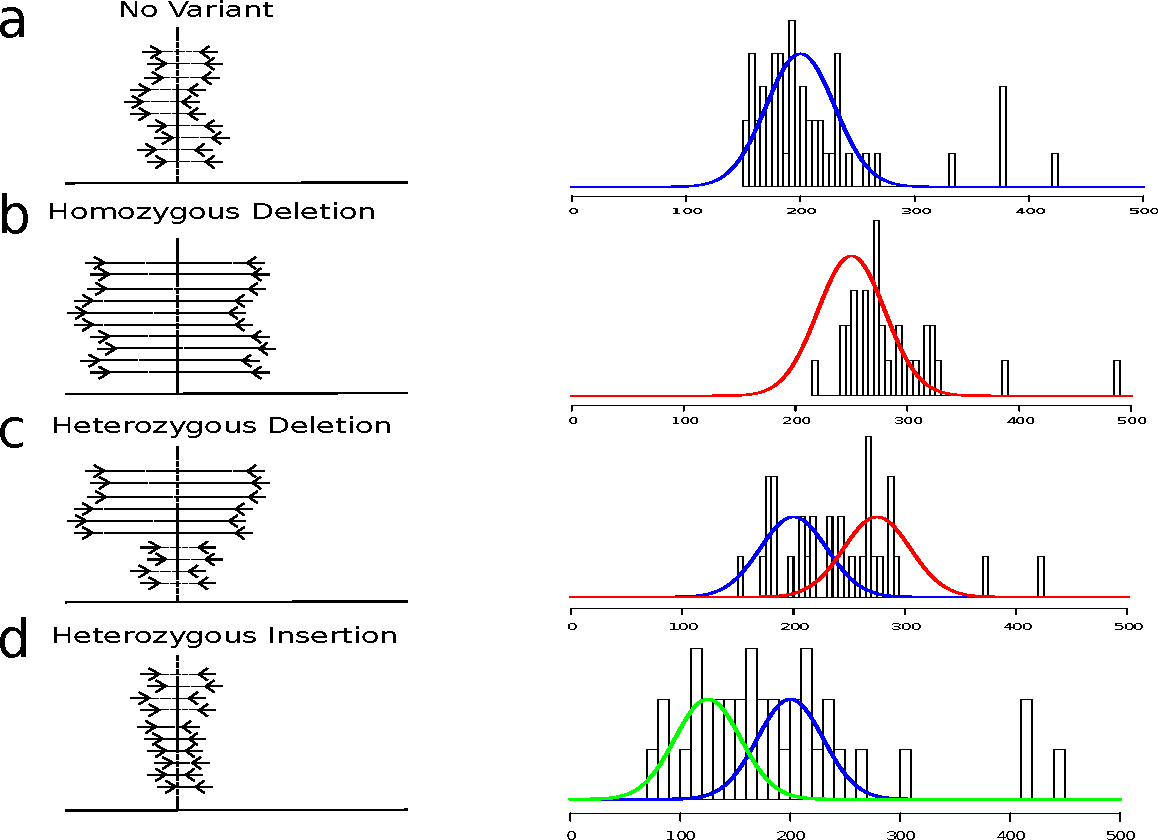
\includegraphics[width=1\textwidth]{/users/cwhelan/insert_size_mixtures.pdf}
\caption{Illustration of insert size mixtures at individual genomic locations. A) there is no variant present at the location indicated by the vertical line (left), so the mix of insert sizes (right) follows the expected distribution of the library centered at 200bp, with a small amount of noise coming from low-quality mappings. B) a homozygous deletion of 50bp at the location has shifted the distribution of observed insert sizes. C) A heterozygous deletion at the location causes a mixture of normal and long insert sizes to be detected. D) A heterozygous small insertion shifts a portion of the mixture to have lower insert sizes.}
\label{insert_size_mixes}
\end{figure}

To handle incorrect and ambiguous mappings, we assume that in general they will not form normally distributed clusters in the same way that correct mappings will, and therefore use an outlier detection technique to filter the observed insert sizes for each location. We sort the observed insert sizes and define as an outlier an observation whose $k$th nearest neighbor is more than $n\sigma$ distant, where $k = 3$ and $n = 5$. In addition, we rank all observations by the estimated probability that the mapping is correct and use an \emph{adaptive quality cutoff} to filter observations: we discard all observations where the estimated probability the mapping is correct is less than the score of the maximum quality observation minus a constant $c$. This allows the use of more uncertain mappings in repetitive regions of the genome while restricting the use of low-quality mappings in unique regions. Defining $\textsc{Mismatches}(a)$ to be the number of mismatches between a read and the reference genome in the alignment $a$, we approximate the probability $p^{k}_c$ of each end alignment being correct by:

\[ p^{k}_c(a^{k}_{m,i}) = \frac{\exp({-\textsc{Mismatches}(a^{k}_{m,i})/2)}}{\sum_j{\exp(-\textsc{Mismatches}(a^{k}_{m,j})/2)}} \]

And then multiply $p_c(a^{1}_{m,i})$ and $p_c(a^{2}_{m,i})$ to approximate the likelihood that the pair is mapped correctly.

We fit the parameters of the GMM using the Expectation-Maximization algorithm. Let $Y = y_{1,2, \ldots m}$ be the observed insert sizes at each location after filtering, and say the library has mean fragment size $\mu$ with standard deviation $\sigma$. We initialize the two components to have means $\mu$ and $\bar{Y}$, set the standard deviation of both components to $\sigma$, and set $\alpha = .5$. In the E step, we compute for each $y_i$ and GMM component $j$ the value $\gamma_{i,j}$, which is the normalized likelihood that $y_i$ was drawn from component $j$. We also compute $n_j = \sum_i{\gamma_{i,j}}$, the relative contributions of the data points to each of the two distributions. In the M step, we update $\alpha$ to be $n_2 - \left|Y\right|$, and set the mean of the second component to be $\frac{\sum_m{\gamma_{m,2}y_m}}{n_2}$. We treat the variance as fixed and do not update it, since under our assumptions the standard deviation of each component should always be $\sigma$. We repeat the E and M steps until convergence, or until a maximum number of steps has been taken.

The features generated for each location $l$ include the log-likelihood ratio of the filtered observed data points under the fit GMM to their likelihood under the distribution $N(\mu,\sigma)$, the final value of the mixing parameter $\alpha$, and $\mu'$, the estimated mean of the second GMM component.

\item[\sc{PostProcess}] We convert our features along the genome to insertion and deletion calls by first extracting contiguous genomic loci where the log-likelihood ratio of the two models is greater than a given threshold. To eliminate noise we apply a median filter with window size 5. We end regions when $\mu'$ changes by more than 60bp ($2\sigma$), and discard regions where the average value of $\mu'$ is less than $\mu$ or where the length of the region differs from $\mu'$ by more than $\mu$.
\end{description}

A diagram of the Cloudbreak algorithm working on a simple example is shown in Figure \ref{algorithm_example}.

\begin{figure}
\centering
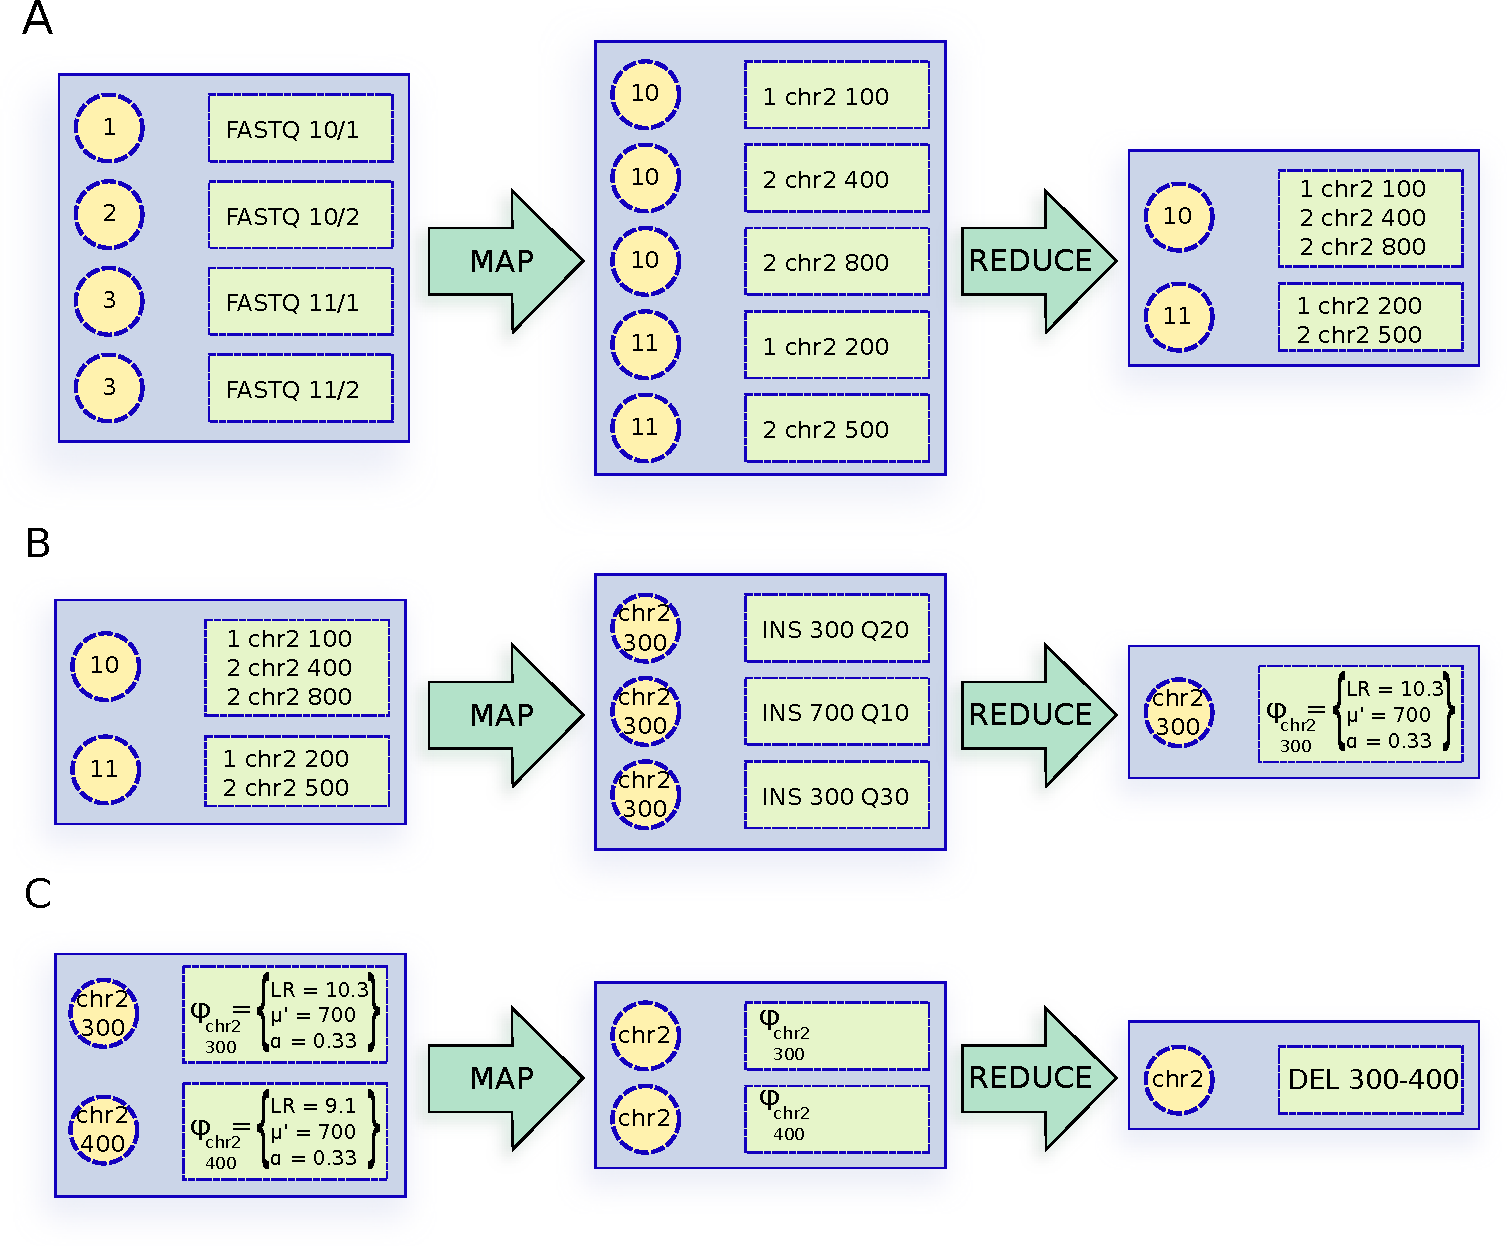
\includegraphics[width=1\textwidth]{cloudbreak_mapred_diagram.pdf}
\caption{An example of the Cloudbreak MapReduce algorithm. A) In the first MapReduce job, mappers scan input reads in FASTQ format and execute an alignment program in single-ended mode to generate aligned reads. Reducers gather all alignments for both reads in each pair. B) In the second MapReduce job, mappers first emit information about each read pair (in this case the insert size and quality) keys indicating the genomic location spanned by that pair. Only one genomic location is diagrammed here for simplicity. Reducers then compute features for each location on the genome by fitting a GMM to the distribution of spanning insert sizes. C) Mappers group all emitted features by their chromosome, and reducers find contiguous blocks of features that indicate the presence of a deletion.}
\label{algorithm_example}
\end{figure}

\section{Results}\label{results}

We compared the performance of Cloudbreak for detecting deletions and insertions to a selection of popular tools: the RP method Breakdancer \autocite{Chen:2009p3}, GASVPro, an RP method that integrates RD signals and ambiguous mappings to increase sensitivity and specificity \autocite{Sindi:2012kk}, the SR method Pindel \autocite{Ye:2009p2}, and the hybrid RP-SR method DELLY \autocite{Rausch:2012he}. We also attempted to evaluate MoDIL on the same data. All of these methods detect deletions; in addition Breakdancer, Pindel, and MoDIL are capable of detecting insertions. In each case we use default parameters and attempt to follow the recommend pipelines for alignment for each tool (See Methods for details).

We use the following criteria to define a true prediction given a gold standard set of deletion and insertion variants to test against: A predicted deletion is counted as a true positive if a) it overlaps with a deletion from the gold standard set, b) the length of the predicted call is within 300bp (the library fragment size in both our real and simulated libraries) of the length of the true deletion, and c) the true deletion has not been already been discovered by another prediction from the same method. For evaluating insertions, each algorithm produces insertion predictions that define an interval in which the insertion is predicted to have occurred with start and end coordinates $s$ and $e$ as well as the predicted length of the insertion, $l$. The true insertions are defined in terms of their actual insertion coordinate $i$ and their actual length $l_a$. Given this information, we modify the overlap criteria in a) to include overlaps of the intervals $\langle s,\max{\left(e,s+l\right)} \rangle$ and $\langle i,i+l_a \rangle$. In this study we are interested in detecting events larger than 40bp, because with longer reads, smaller events can be more easily discovered by examining gaps in individual reads. Both Pindel and MoDIL make many calls with a predicted event size of under 40bp, so we remove those calls from the output sets of those programs. Finally, we exclude from consideration calls from all approaches that match a true deletion of less than 40bp where the predicted variant length is less than or equal to 75bp in length.

It should be noted that the methods tested here vary in their breakpoint resolution: SR methods have higher resolution than RP methods. Cloudbreak sacrifices additional resolution (by dividing the genome into 25bp windows); we strive however to increase sensitivity and specificity in the hopes that such calls could still be useful even if their resolution is limited. This seems reasonable to us given the possibility of pipelines in which RP calls are refined by SR mappings or local assembly methods.

\subsection{Tests with Simulated Data}

As has been observed elsewhere, there is no available test set of real Illumina sequencing data from a sample that has a complete annotation of structural variations from the reference. Therefore, testing with simulated data is important to fully characterize an algorithm's performance characteristics. On the other hand, it is important that the simulated data contain realistic SVs that follow patterns of SVs observed in real data. To address this, we took one of the most complete lists of SVs from a single sample available, the list of homozygous insertions and deletions from the genome of J. Craig Venter \autocite{Levy:2007fb}. Since there are relatively few heterozygous insertions and deletions annotated in the Venter genome, we randomly assigned each variant to be either homozygous or heterozygous and applied them to one or both of two copies of the human GRCh36 chromosome 2 reference sequence. We then simulated paired Illumina reads from these modified references using \emph{dwgsim} from the DNAA software package\footnote{\url{http://sourceforge.net/apps/mediawiki/dnaa/}}. We simulated 100bp reads with a mean fragment size of 300bp and a standard deviation of 30bp, and generated 15X coverage for each modified sequence. Pooling the reads from both simulations gives 30X coverage for a diploid sample with a mix of homozygous and heterozygous insertions and deletions.

\begin{figure}
\centering
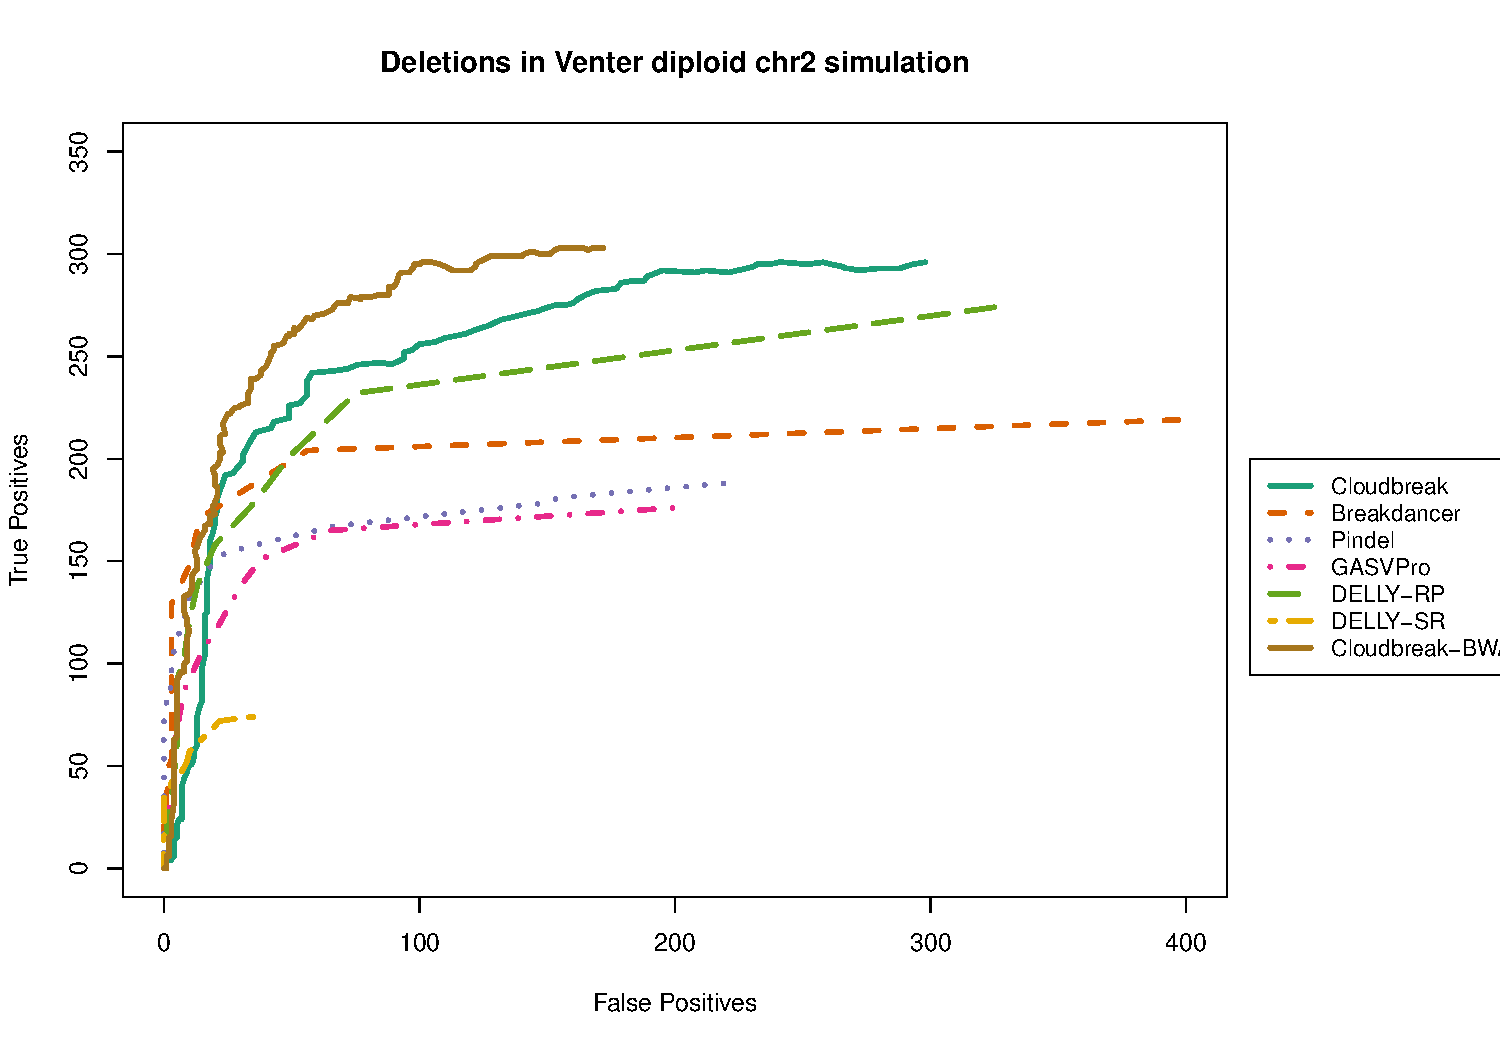
\includegraphics[width=0.75\textwidth]{/Users/cwhelan/Documents/gene_rearrange/svpipeline/venter_chr2_allindels_100bp_dip/CHR2SIM_DELS_ROC.pdf}
\caption{ROC curve of deletion prediction performance on a simulated set of reads giving diploid coverage of 30X on human chromosome 2 with insertions and deletions from the Venter genome added to one or both haplotypes. Thresholds vary by: Cloudbreak - likelihood ratio; Breakdancer, DELLY, GASVPro - number of supporting read pairs; Pindel - simple score.}
\label{chr2DeletionsRoc}
\end{figure}

\begin{figure}
\centering
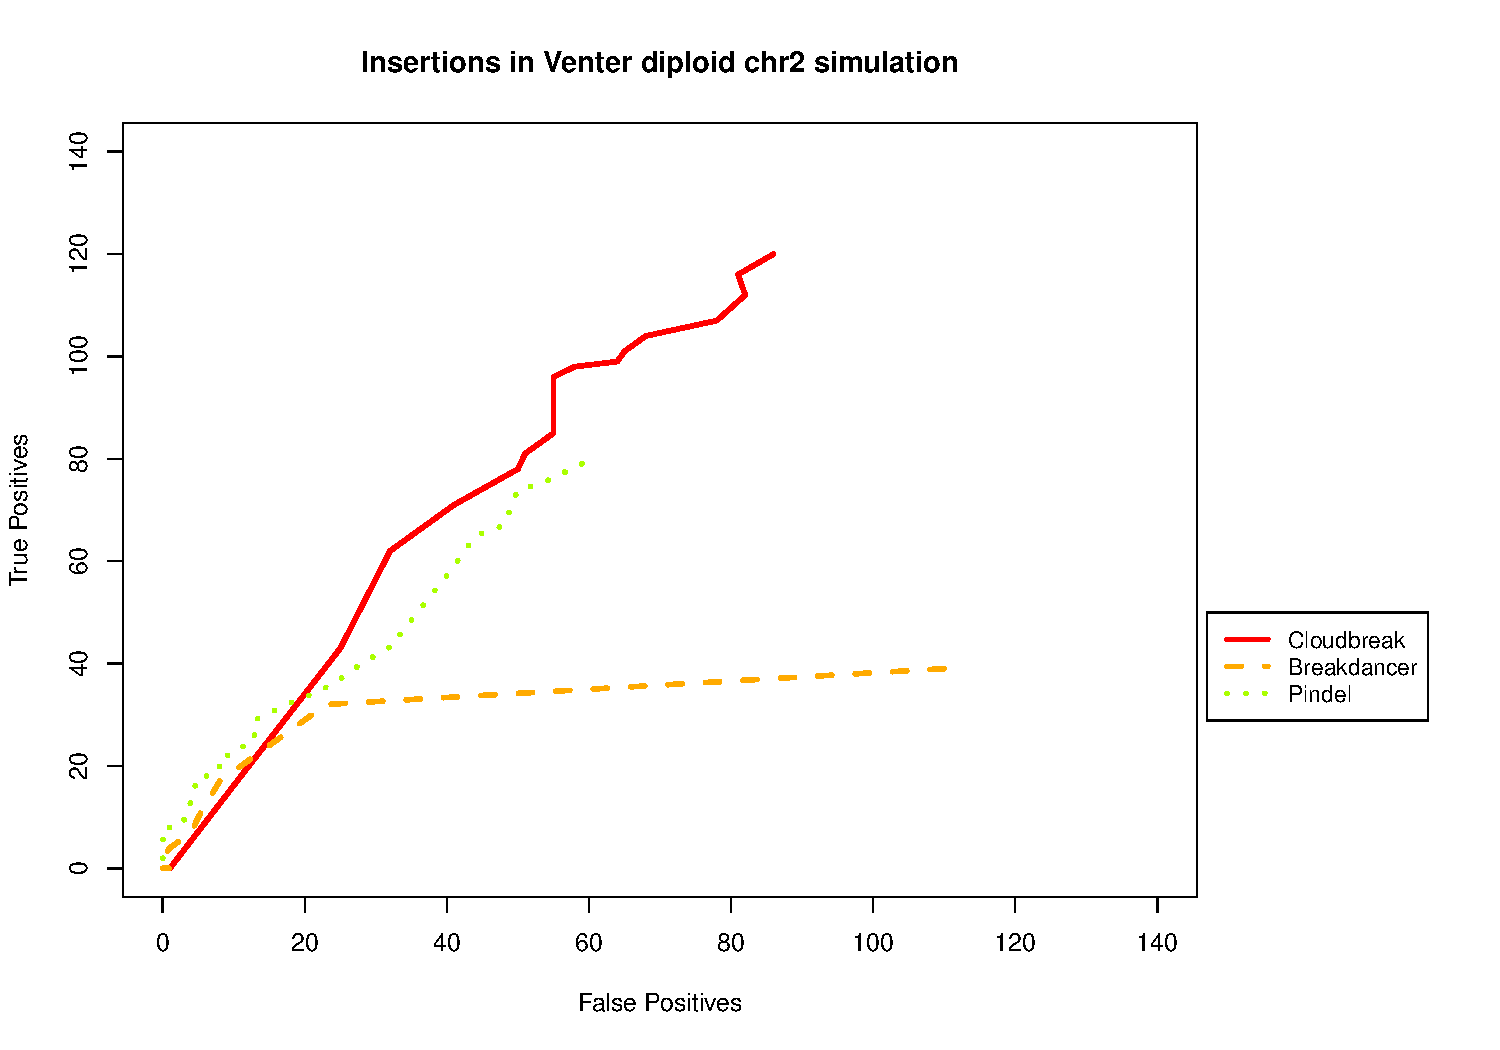
\includegraphics[width=0.75\textwidth]{/Users/cwhelan/Documents/gene_rearrange/svpipeline/venter_chr2_allindels_100bp_dip/CHR2SIM_INS_ROC.pdf}
\caption{ROC curve of insertion prediction performance on the chromosome 2 simulated data set.}
\label{chr2InsertionsRoc}
\end{figure}

Figure \ref{chr2DeletionsRoc} shows an ROC plot of the performance of each algorithm for detecting deletions on the simulated data set. All approaches show excellent specificity at high thresholds in this simulation. Cloudbreak provides the greatest specificity at higher levels of sensitivity, followed by DELLY. The output which we obtained from MoDIL did not have a threshold that could be varied to correlate with the tradeoff between precision and recall; therefore it is not included in this figure. A ROC curve for insertion prediction performance is shown in Figure \ref{chr2InsertionsRoc}.

Choosing the correct operating point or threshold can be difficult when operating on a new data set, but the use of simulated data and ROC curves allows for some investigation of the performance characteristics of algorithms at varying levels. First, we used the ROC curves to attempt to characterize the predictions made by each algorithm when a low false discovery rate is required. Table \ref{chr2DeletionPredsFDR10} shows the total number of simulated deletions found by each tool when choosing a threshold that gives an FDR closest to 10\% based on the ROC curve, representing cutoffs of 2.22 log likelihood ratio for Cloudbreak, 4 supporting read pairs for Breakdancer, 11 supporting read pairs for GASVPro, 7 supporting read pairs for DELLY, and a simple score of 13 for Pindel. Cloudbreak shows good performance at detecting deletions in all size classes, and finds more medium and large deletions than the other approaches. Pindel exclusively identifies a large number of small (40bp-100bp) deletions, as is expected for a split-read method. Performance on insertions never reached a level with an FDR of 10\%, so insertion predictions are not included in this table.

\begin{table}
\begin{center}
\begin{tabular}{rrrrrr}
  \hline
 & 40-100bp  & 101-250bp  & 251-500bp & 501-1000bp & $>$ 1000bp \\ 
 Total Number & 224 &  84 & 82 &  31 & 26\\ 
  \hline
  Cloudbreak  &  47 (  7)  &  52 (\textbf{  3}) &  \textbf{ 57} (\textbf{  5}) & \textbf{ 12} (\textbf{  4}) & \textbf{ 15} (\textbf{0}) \\ 
  Breakdancer &  52 ( 10)  &  49 (\textbf{  3}) &   49 (0) &   7 (0) &  14 (\textbf{0}) \\ 
  GASVPro     &  35 (  4)  &  26 (0) &   26 (0) &   2 (0) &   6 (\textbf{0}) \\ 
  DELLY       &  22 (  2)  & \textbf{ 56} (  2) &   40 (0) &   8 (0) &  12 (\textbf{0}) \\ 
  Pindel      & \textbf{ 60} (\textbf{ 34})  &  16 (0) &   41 (  1) &   1 (0) &  12 (\textbf{0})\\ 
   \hline
\end{tabular}
\end{center}
\caption{The number of simulated deletions in the 30X diploid chromosome 2 with Venter indels found by each tool at a 10\% FDR, as well as the number of those deletions that were discovered exclusively by each tool (in parentheses). The total number of deletions in each size class in the true set of deletions is shown in the second row of the header.}
\label{chr2DeletionPredsFDR10}
\end{table}

We also characterized the predictions made by each algorithm at the operating point which gives them maximum sensitivity. For Cloudbreak we chose an operating point at which marginal improvements in sensitivity became very low. The results for both deletion and insertion predictions are summarized in Table \ref{chr2DeletionAndInsertionPredsMaxSensitivity}. MoDIL and Cloudbreak exhibited the greatest recall for deletions. Cloudbreak has high precision and recall for deletions at this threshold, and surprisingly discovers more small deletions than Pindel. For insertions, Cloudbreak shows excellent precision, although recall is low for all four approaches, with Cloudbreak and Pindel showing the highest recall rates. Cloudbreak again identifies the most small variants. Pindel is the only tool which can consitently identify large insertions, as insertions larger than the library insert size do not produce mapping signatures detectable by read-pair mapping.


\begin{table}
\begin{center}
\begin{tabular}{r|rrr|rrrrr}
  \cline{2-9}
   &                     & Prec. & Recall & 40-100bp  & 101-250bp  & 251-500bp & 501-1000bp & $>$ 1000bp \\ 
\hline
\multirow{7}{*}{\begin{sideways}Deletions\end{sideways}} & Total Number &          &           & 224 &  84 & 82 &  31 & 26\\ 
  \hline
\cline{2-9}
&  Cloudbreak    &  0.532 & \textbf{0.66} & \textbf{146} (  6)  &  58 (\textbf{  4}) &   62 (  1) &  14 (  1) &  15 (0) \\ 
&  Breakdancer   &  0.356 & 0.49 &  89 (0)  &  54 (0) &   53 (0) &   8 (0) &  15 (0) \\ 
&  GASVPro        & 0.146 & 0.432 &  83 (  2)  &  32 (0) &   55 (0) &   8 (0) &  15 (0) \\ 
&  DELLY-RP           & 0.457 & 0.613 & 114 (  8)  & \textbf{ 68} (  2) &  \textbf{ 66} (0) &   9 (0) &  17 (0) \\ 
&  DELLY-SR           & \textbf{0.679} & 0.166 & 0 (0)  &   3 (0) &   49 (0) &   6 (0) &  16 (0) \\ 
&  Pindel           & 0.462 & 0.421 &  96 (\textbf{ 13})  &  24 (0) &   48 (0) &   5 (0) &  15 (0)\\ 
&  MoDIL           & 0.132  & \textbf{0.66} & 123 (  5)  &  66 (  2) &  \textbf{ 66} (\textbf{  7}) & \textbf{ 17} (\textbf{  6}) & \textbf{ 23} (\textbf{  8})\\ 
   \hline
\multirow{5}{*}{\begin{sideways}Insertions\end{sideways}} & Total Number &          &           & 199 &  83 & 79 &  21 & 21\\ 
\cline{2-9}
&  Cloudbreak   &\textbf{0.705} & \textbf{0.196}  & \textbf{ 67} ( 24)  &   8 (  3) &    3 (  1) &   1 (0) & 0 (0) \\ 
&  Breakdancer & 0.262 & 0.0968  &  23 (  8)  & \textbf{ 14} (\textbf{  9}) &    2 (  1) & 0 (0) & 0 (0) \\ 
&  Pindel          & 0.572 & \textbf{0.196} &  52 (\textbf{ 26})  &   5 (  3) &  \textbf{ 10} (\textbf{ 10}) & \textbf{  3} (\textbf{  3}) & \textbf{  9} (\textbf{  9})\\ 
&  MoDIL          & 0.186 & 0.0521 &  14 (  1)  &   4 (  1) &    1 (0) &   2 (  1) & 0 (0)\\ 
\hline
\end{tabular}
\end{center}
\caption{The precision and recall of each tool for the simulated deletions and insertions in the 30X diploid chromosome 2 with Venter indels at maximum sensitivity, as well as the number of those variants discovered in each size class. Variants exclusively predicted by one tool are shown in parentheses. The total number of variants in each size class in the true set of deletions and insertions is shown in the first row of each section.}
\label{chr2DeletionAndInsertionPredsMaxSensitivity}
\end{table}

\subsection{Tests with Biological Data}

We downloaded a data set of reads taken from a DNA sample of Yoruban individual NA18507, experiment ERX009609 from the Sequence Read Archive.\footnote{\url{http://sra.dnanexus.com/experiments/ERX009609}} This sample was sequenced on the Illumina Genome Analyzer II platform with 100bp paired end reads and a mean fragment size (minus adapters) of 300bp, with a standard deviation of 15bp. The sample was sequenced to a depth of approximately 37X coverage.

To create a gold standard set of insertions and deletions to test against, we pooled annotated variants discovered by three previous studies on the same sample. These included data from the Human Genome Structural Variation Project\footnote{\url{http://hgsv.washington.edu/general/download/SNPs_DIPs/}} reported by \textcite{Kidd:2008p926}, a survey of small indels conducted by \textcite{Mills:2011fi}, and insertions and deletions from the merged call set of the phase 1 release of the 1000 Genomes Project \autocite{GenomesProjectConsortium:2012co} which were genotyped as present in NA18507. We merged any overlapping calls of the same type into the region spanned by their unions. It should be noted that the 1000 Genomes call set was partially produced using DELLY and Breakdancer, and therefore those calls are ones that those tools are sensitive to, biasing this test in their favor. We were unable to run MoDIL on the whole-genome data set due to the estimated runtime and storage requirements.

\begin{figure}
\centering
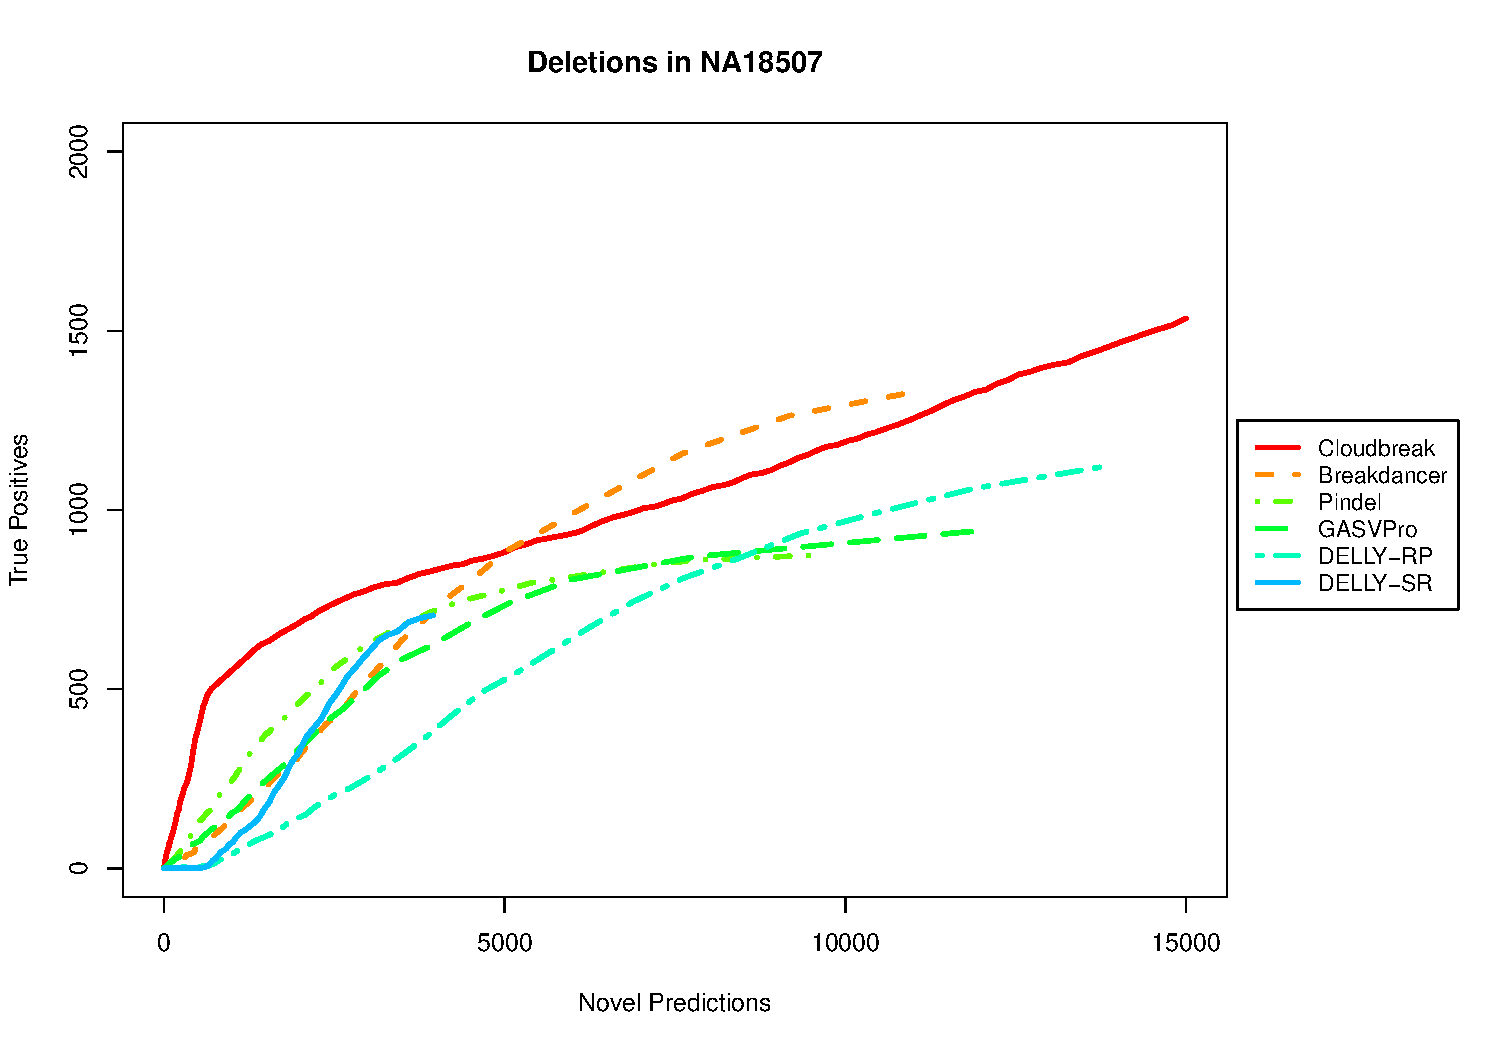
\includegraphics[width=0.75\textwidth]{/Users/cwhelan/Documents/gene_rearrange/svpipeline/NA18507/NA18507_DELS_ROC.pdf}
\caption{ROC curve of deletion prediction performance on the 37X NA18507 sample, tested against the combined gold standard deletion set taken from \textcite{Kidd:2008p926}, \textcite{Mills:2011fi}, and \textcite{GenomesProjectConsortium:2012co}.}
\label{NA18507DeletionsRoc}
\end{figure}

Figure \ref{NA18507DeletionsRoc} shows the performance of each algorithm on the NA18507 data set when compared against the gold standard deletion set, using the same rules for a match as described in the previous section. All algorithms show far less specificity for the gold standard set than they did for the true deletions in the single chromosome simulation, although it is difficult to tell how much of the difference is due to the added complexity of real data and a whole genome, and how much is due to missing deletions in the gold standard set that are actually present in the sample. Cloudbreak is the best performer at more stringent thresholds, and remains near the top at higher sensitivity levels.

We then tested the predictions made by each algorithm using the same cutoffs that yielded a 10\% FDR on the simulated chromosome 2 data set, adjusted proportionally for the difference in coverage from 30X to 37X. The precision and recall with respect to the gold standard deletion set, as well as the performance of each algorithm at predicting each size class at those thresholds, is shown in Table \ref{NA18507DeletionPreds}. Cloudbreak has the greatest sensitivity of any tool at these thresholds, identifying the most variants in each size class.

\begin{table}
\begin{center}
\begin{tabular}{rrr|rrrrr}
  \hline
 & Prec. & Recall & 40-100bp & 101-250bp & 251-500bp & 501-1000bp & $>$ 1000bp \\ 
Total Number & & & 7,466 & 235 & 218 & 110 & 375 \\
  \hline
Cloudbreak & 0.11 & \textbf{0.13} & \textbf{371} (\textbf{127})  & \textbf{146} (\textbf{ 15}) &  \textbf{177} (\textbf{  9}) & \textbf{ 95} (\textbf{  3}) & \textbf{301} (\textbf{ 19}) \\ 
Breakdancer & 0.122 & 0.112 & 261 ( 41)  & 132 (  6) &  167 (0) &  92 (0) & 288 (  2) \\  
  GASVPro & 0.135 & 0.0449 & 120 ( 28)  &  38 (  3) &   80 (0) &  29 (0) & 110 (0) \\ 
  DELLY & 0.0824 & 0.091 & 143 (  8)  & 125 (  4) &  158 (  1) &  83 (  1) & 256 (  3) \\ 
  Pindel & \textbf{0.16} & 0.0685 & 149 ( 12)  &  57 (0) &  140 (0) &  58 (0) & 172 (0) \\ 
   \hline
\end{tabular}
\end{center}
\caption{The precision and recall with respect to the gold standard set of each tool on the NA18507 data, as well as the number of deletions in each size class found. The same cutoffs were used as for the simulated data as in Table \ref{chr2DeletionPredsFDR10}, adjusted for the difference in coverage from 30X to 37X.}
\label{NA18507DeletionPreds}
\end{table}

\begin{figure}
\centering
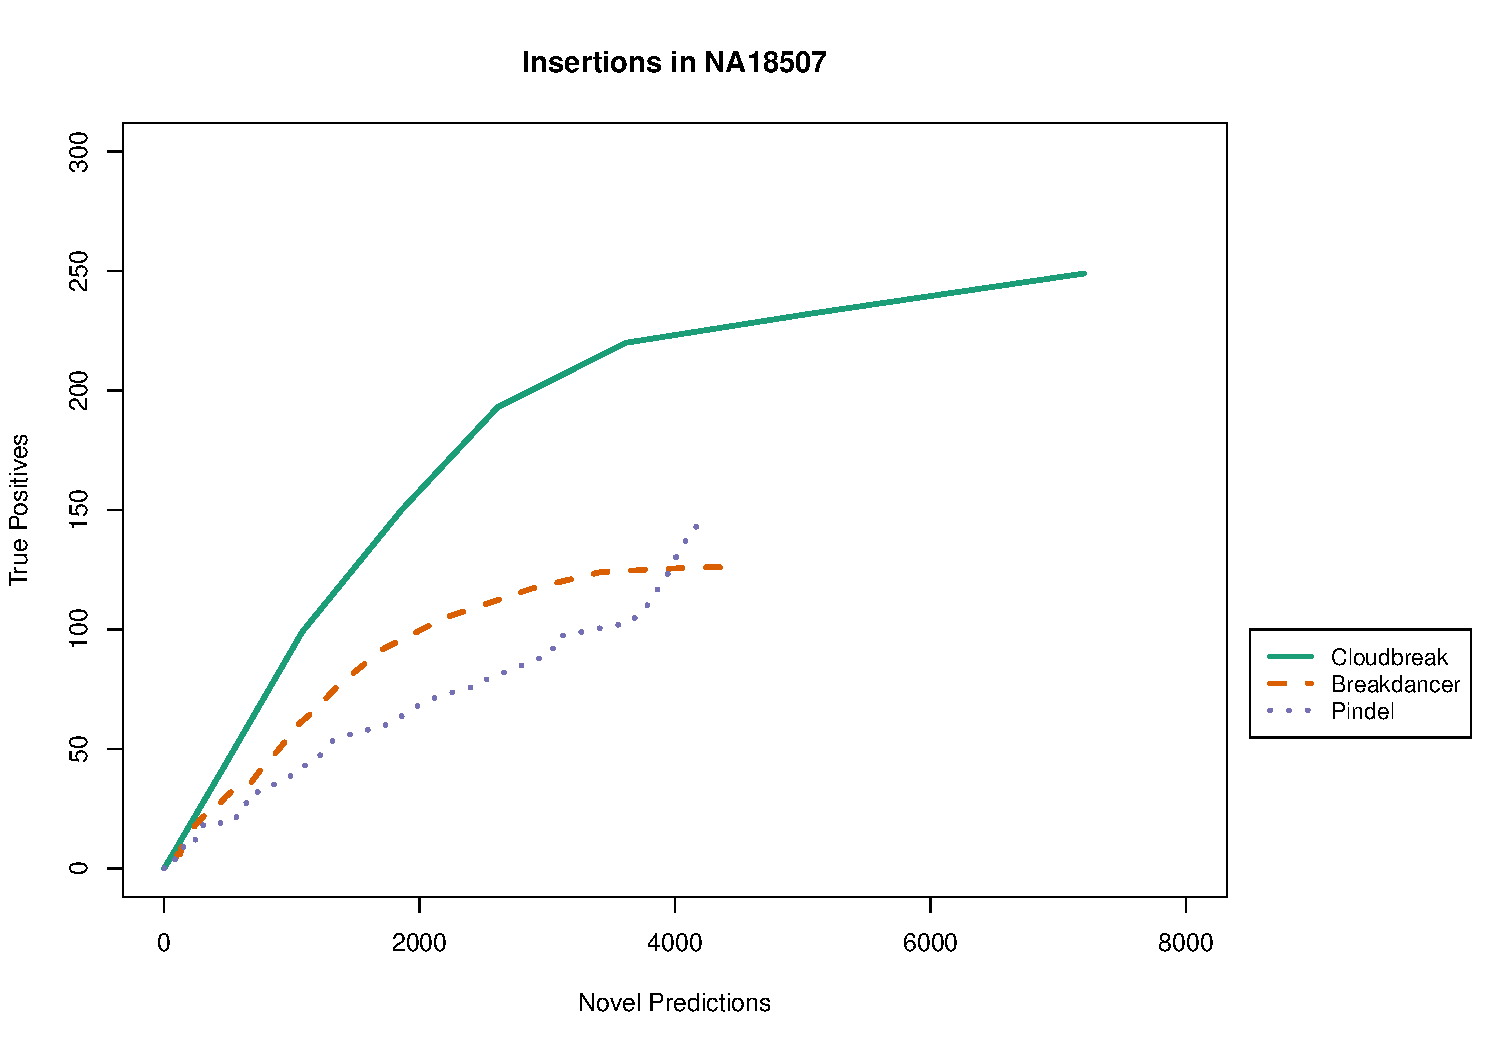
\includegraphics[width=0.75\textwidth]{/Users/cwhelan/Documents/gene_rearrange/svpipeline/NA18507/NA18507_INS_ROC.pdf}
\caption{ROC curve of insertion prediction performance on the 37X NA18507 sample.}
\label{NA18507InsertionsRoc}
\end{figure}

A similar ROC-like curve for insertions on the NA18507 data set is shown in Figure \ref{NA18507InsertionsRoc}. The number of insertions detected at maximum sensitivity for the three algorithms is shown in Table \ref{NA18507InsertionPreds}, along with their precision and recall at that threshold. Cloudbreak has the greatest recall, identifying twice as many short insertions as Pindel, while Pindel has the best precision.

\begin{table}
\begin{center}
\begin{tabular}{rrr|rrrrr}
  \hline
 & Prec. & Recall & 40-100bp & 101-250bp & 251-500bp & 501-1000bp \\ 
Total Number & & & 536 & 114 & 45 & 1 \\
  \hline
Cloudbreak & 0.0268 & \textbf{0.391} & \textbf{246} (\textbf{ 83})  &  25 (  9) &    1 (0) & 0 (0) \\ 
Breakdancer & 0.0281 & 0.181 &  97 ( 11)  & \textbf{ 27} (  9) &    2 (  1) & 0 (0) \\  
  Pindel & \textbf{0.0387} & 0.239 & 144 ( 41)  &  14 (\textbf{ 12}) &  \textbf{  7} (\textbf{  7}) & \textbf{  1} (\textbf{  1})  \\ 
   \hline
\end{tabular}
\end{center}
\caption{The precision and recall with respect to the gold standard set of insertions for each tool on the NA18507 data, as well as the number of insertions in each size class found, at maximum sensitivity.}
\label{NA18507InsertionPreds}
\end{table}

\subsection{Performance in Repetitive Areas}

We analyzed the predictions made by Cloudbreak to determine whether any particular class of deletion event was contributing to its performance. We found that Cloudbreak shows particularly strong performance in detecting deletions that overlap RepeatMasker-annotated elements in both the simulated and NA18507 data sets. Table \ref{deletionRepmaskpreds} shows the number of deletions that overlap repeats at the 10\% FDR cutoff described above. In the NA18507 data set, Cloudbreak identifies 15\% more repeat-overlapping variants than the nearest competitor, Breakdancer. Since deletions and other SVs are enriched in repetitive regions of the genome in both of our data sets, this contributes greatly to Cloudbreak's performance, and demonstrates the value in considering as many possible mappings of ambiguously mapping reads as possible. Performance on insertions is displayed in Table \ref{insertionRepmaskpreds}; again, Cloudbreak identifies more events that lie in repetitive regions than the other tools.

\begin{table}
\begin{center}
\begin{tabular}{rrr|rr}
 & \multicolumn{2}{c}{Simulated Data} & \multicolumn{2}{c}{NA18507} \\
\hline
 &  Non-repeat & Repeat  &  Non-repeat & Repeat \\ 
 Total Number & 120 & 327 & 553 & 7851 \\ 
  \hline
  Cloudbreak  &  25 (  2) & \textbf{158} ( 17) & \textbf{220} (\textbf{ 49}) & \textbf{870} (\textbf{124}) \\ 
  Breakdancer & \textbf{ 29} (  6) & 142 (  7) & 186 ( 19) & 754 ( 30) \\
  GASVPro     &  16 (  2) &  79 (  2) &  75 (  9) & 302 ( 22) \\
  DELLY       &  21 (  2) & 117 (  2) & 147 (  9) & 618 (  8) \\
  Pindel      &  18 (\textbf{  9}) & 112 (\textbf{ 26}) & 103 (  4) & 473 (  8) \\ 
   \hline
\end{tabular}
\end{center}
\caption{Detected deletions on the simulated and NA18507 data sets identified by each tool, broken down by whether the deletion overlaps with a RepeatMasker-annotated element.}
\label{deletionRepmaskpreds}
\end{table}

\begin{table}
\begin{center}
\begin{tabular}{rrr|rr}
 & \multicolumn{2}{c}{Simulated Data} & \multicolumn{2}{c}{NA18507} \\
\hline
 &  Non-repeat & Repeat  &  Non-repeat & Repeat \\ 
 Total Number & 133 & 270 & 341 & 355 \\ 
  \hline
  Cloudbreak  &  21 (  4) & \textbf{ 58} ( 24) & \textbf{137} (\textbf{ 37}) & \textbf{135} (\textbf{ 55}) \\ 
  Breakdancer &  17 (  7) &  22 ( 11) &  82 ( 12) &  44 (  9) \\
  Pindel      & \textbf{ 25} (\textbf{ 18}) &  54 (\textbf{ 33}) &  84 ( 36) &  82 ( 25) \\ 
  MoDIL      &   5 (0) &  16 (  3) & NA & NA \\ 
   \hline
\end{tabular}
\end{center}
\caption{Detected insertions in the simulated and NA18507 data sets identified by each tool, broken down by whether the insertion occurs in a RepeatMasker-annotated element.}
\label{insertionRepmaskpreds}
\end{table}

\subsection{Genotyping Variants}

Since Cloudbreak explicitly fits a mixture of insert size distributions at each location, and each component of the mixture represents an allele containing or not containing an insertion or deletion, it should be possible to use the parameters of the fit GMM to infer the genotype of each predicted variant, assuming that our pipeline is capturing all relevant read mappings near the locus of the variant. To test this, we attempted to classify the true positive Cloudbreak predictions described above for both the simulated and biological data sets. Because we simulated a diploid genome, we had genotypes for the simulated data readily available. For benchmarking genotyping of deletions in the real dataset, we only considered the deletions from the 1000 Genomes Project data set, which had been genotyped as part of the Phase 1 release using the population-scale SV detection algorithm Genome STRiP \autocite{Handsaker:2011ki}. We found that we could use $\alpha$, the mixing parameter that controls the weight of the two components in the GMM, to accurately predict deletion genotypes. By setting a simple cutoff of .35 on the average value of $\alpha$ in each Cloudbreak prediction, we were able to achieve 88.1\% and 96.5\% accuracy in predicting the genotype of the true positive deletions we detected at our 10\% FDR threshold in the simulated and real data sets respectively. Table \ref{deletionGenotypeaccuracy} shows confusion matrices for the two samples using this classifier. For insertions, none of the three input sets that made up the gold standard for NA18507 contained a sufficient number of insertion rates that meet our size threshold that also had genotyping information. Of the 79 insertions detected by Cloudbreak on the simulated data set, 13 were heterozygous. Using the same cutoff of .35 on $\alpha$, Cloudbreak correctly classified 62 of the 66 homozygous insertions and 10 of the 13 heterozygous insertions discovered, for an overall accuracy rate of 91\%.

\begin{table}
\begin{center}
\begin{tabular}{r|r|rr|rr|}
\multicolumn{2}{c}{}  & \multicolumn{4}{c}{Actual Genotypes} \\
\multicolumn{2}{c}{}  & \multicolumn{2}{c}{Simulated Data} & \multicolumn{2}{c}{NA18507} \\
\cline{3-6}
\multicolumn{2}{c|}{} &  Homozygous & Heterozygous & Homozygous & Heterozygous \\ 
\cline{2-6}
\multirow{2}{*}{\shortstack{Predicted \\ Genotypes}} & Homozygous & 100 & 4 &  77 & 12 \\
 & Heterozygous & 7 & 72 &  3 & 338 \\
\cline{2-6}
\end{tabular}
\end{center}
\caption{Confusion matrices for the predicted genotype of deletions found by Cloudbreak on both the simulated and NA18507 data sets.}
\label{deletionGenotypeaccuracy}
\end{table}

\subsection{Runtimes}

We implemented and executed Cloudbreak on a 56-node Hadoop cluster, with 636 map slots and 477 reduce slots. Not including alignment time, we were able to process the Chromosome 2 simulated data in under 6 minutes, and the the NA18507 data set in under 40 minutes. For the simulated data set we used 100 reducers for the compute SV features job; for the real data set we used 300. The bulk of Cloudbreak's execution is spent in the feature generation step. Extracting deletion and insertion calls take under two minutes each for both the real and simulated data sets; the times are equal because each reducer is responsible for processing a single chromosome, and so the runtime is bounded by the length of time it takes to process the largest chromosome. 

In table \ref{runtimes} we display a comparison of runtimes on the real and simulated data sets for all of the tools evaluated in this work. Each tool varies in the amount of parallelization supported. We report runtimes for tools run in their default single-threaded mode, as well as for levels of parallelization achievable with basic scripting, noting that one of the key advantages of Hadoop/MapReduce is the ability to scale parallel execution to the size of the available compute cluster without any custom programming. Pindel allows multi-threaded operation on multicore servers. Pindel and Breakdancer allow processing of a single chromosome in one process, so it is possible to execute all chromosomes in parallel on a cluster that has a job scheduler and shared filesystem. Breakdancer has an additional preprocessing step (\texttt{bam2cfg.pl}) which runs in a single thread. DELLY suggests splitting the input BAM file by chromosome, after which a separate DELLY process can be executed on the data for each chromosome; splitting a large BAM file is a time consuming process and consumes most of the time in this parallel workflow, in fact making it faster to run in single-threaded mode. GASVPro allows parallelization of the MCMC component for resolving ambiguously mapped read pairs; however, this requires a significant amount of custom scripting, and we did not find that the MCMC module consumed most of the runtime in our experiments, so we do not attempt to parallelize this componen. The MoDIL distribution contains a set of scripts that can be used to submit parallel jobs to the SGE scheduling engine or modified for other schedulers; we adapted these for use in our cluster.

In parallel execution, the total time to execute is bounded by the runtime of the longest-running process. In the case of chromosome-parallelizable tools including Breakdancer, Pindel, and DELLY, this is typically the process working on the largest chromosome.\footnote{We note that one Breakdancer process, handling an unplaced contig in the hg19 reference genome, never completed in our runs and had to be killed manually; we exclude that process from our results.} In the case of MoDIL's run on the simulated data, we found that the different processes varied widely in their execution times, likely caused by regions of high coverage or with many ambiguously mapped reads. Cloudbreak mitigates this problem during the time-consuming feature generation process by using Hadoop partitioners to randomly assign each genomic location to one of the set of reducers, ensuring that the work is evenly distributed across all processes. This distribution of processing across the entire cluster also server to protect against server slowdowns and hardware failures - for example, we were still able to complete processing of the NA18507 data set in under 50 minutes during a run where one of the compute nodes was rebooted midway through the feature generation job.

\begin{table}
\begin{center}
\begin{tabular}{r|r|rrr|rrr}
\multicolumn{2}{c}{}  & \multicolumn{3}{c}{Simulated Data} & \multicolumn{3}{c}{NA18507} \\
\hline
 & SV Types &  Single CPU & Parallel & Proc. &  Single CPU & Parallel & Proc.  \\ 
  \hline
  Cloudbreak & D,I &   NA    & 308 & 312    & NA         & 2,310 & 636 \\ 
  Breakdancer & D,I,V,T &  653   & NA       & NA          & 134,170 &  5,586 & 84 \\
  GASVPro & D,V   &  3,339  & NA       & NA         & 52,385  & NA & NA \\
  DELLY & D         &  1,964 & NA          & NA      & 30,311  & 20,224 & 84 \\
  Pindel & D,I,V,P         & 37,006 &  4,885     & 8          &  284,932  & 28,587 & 84 \\ 
  MoDIL & D,I        &  NA      & 52,547 & 250 & NA         & NA  & NA\\ 
   \hline
\end{tabular}
\end{center}
\caption{Runtimes (elapsed) on both data sets of each tool tested, in single-processor and parallel mode. For parallel runs, Proc. is the maximum number of simultaneously running processes or threads. All times are in seconds. The types of variants detected by each program are listed with the abbreviations: D - deletion; I - insertion; V - Inversion; P - duplication; T - translocation. Interchromosomal translocations are only detected by Breakdancer in single CPU mode. }
\label{runtimes}
\end{table}

\section{Methods}\label{discussion}

Cloudbreak is a native Java Hadoop application. We deployed Cloudbreak on a 56-node cluster running the Cloudera CDH3 Hadoop distribution, version 0.20.2-cdh3u4. We use snappy compression for MapReduce data. Hadoop's distributed cache mechanism shares the executable files and indices needed for mapping tasks to the nodes in the cluster. To execute the other tools in parallel mode we wrote simple scripts to submit jobs to the cluster using the HTCondor scheduling engine with directed acyclic graphs to describe dependencies between jobs.\footnote{\url{http://research.cs.wisc.edu/htcondor/}}

Simulated reads were aligned to hg18 chromosome 2, and NA18507 reads were aligned to the hg19 assembly. For each evaluated SV detection program we attempt to follow the authors' recommended alignment pipeline, except for MoDIL, for which we used reads aligned with BWA (see below). Cloudbreak alignments were executed in parallel using Hadoop tasks which wrap GEM version 1.362 (beta) in single-ended mode, with parameters \texttt{-e 6 -m 6 -s 2 -q ignore -d 1000 --max-big-indel-length 0},  requesting all hits for a read that are within an edit distance of 6 of the reference, within 2 strata of the best hit, with a maximum of 1000 possible alignments reported for each read. Alignments for the other programs were first aligned using BWA \autocite{Li:2009p836} version 0.6.2-r126, with parameter \texttt{-e 5} to allow for longer gaps in alignments due to the number of small indels near the ends of larger indels in the Venter data set. GASVPro also accepts ambiguous mappings; we extracted read pairs that did not align concordantly with BWA and re-aligned them with Novoalign V2.08.01, with parameters \texttt{-a -r -Ex 1100 -t 250}. 

We ran Breakdancer version 1.1\_2011\_02\_21 in single threaded mode by first executing \texttt{bam2cfg.pl} and then running \texttt{breakdancer\_max} with the default parameter values.  To run Breakdancer in parallel mode we first ran \texttt{bam2cfg.pl} and then launched parallel instances of \texttt{breakdancer\_max} for each chromosome using the \texttt{-o} parameter. We ran DELLY version 0.0.9 with the \texttt{-p} parameter and default values for other parameters. For the parallel run of DELLY we first split the original BAM file with BamTools \autocite{Barnett:2011hm}, and then ran instances of DELLY in parallel for each BAM file. We ran GASVPro version 1.2 using the \texttt{GASVPro.sh} script and default parameters. Pindel 0.2.4t was executed with default parameters in single CPU mode, and executed in parallel mode for each chromosome using the \texttt{-c} option.

\section{Discussion}\label{Discussion}

Over the next few years, due to advances in sequencing technology, genomics data are expected to increase both in volume and in coverage by several orders of magnitude, expanding into the realm referred to as Big Data. In addition, the usage of existing information will increase drastically as research in genomics grows and translational applications are developed, and the data sets are reprocessed and integrated into new pipelines. In order to capitalize on this emerging wealth of genome data, novel computational solutions that are capable of scaling with the increasing number and size of these data sets will have to be developed. 

Among Big Data infrastructures, MapReduce is emerging as a standard framework for distributing computation across compute clusters. In this paper, we introduce a novel conceptual framework for structural variation detection algorithms in MapReduce, based on computing local features along the genome. This framework provides a scalable basis for developing SV detection algorithms, as demonstrated by our development of a distributed deletion-finding algorithm based on fitting a GMM to the distribution of mapped insert sizes spanning each location in the genome. 

On simulated and real data sets, our approach performs well across a wide range of deletion sizes and achieves performance similar to or better than a variety of state-of-the-art structural variation detection algorithms that run on traditional workload clusters and servers. Detection of deletions is an important area of research; \textcite{Mills:2011fi} recently identified over 220 coding deletions in a survey of a large number of individuals, and they note that such variants are likely to cause phenotypic variation in humans. In addition, an increased ability to detect variants in regions of the genome that are repetitive and difficult to align reads to opens up new possibilities in exploring human genetic variation.

In addition to delivering state-of-the-art performance in a RP-based SV detection problem, our approach offers a basis for developing a variety of SV algorithms that are capable of running in a MapReduce pipeline with the power to process vast amounts of data in a cloud or commodity server setting. Using tools like Apache Whirr\footnote{\url{http://whirr.apache.org/}}, it is becoming trivially easy to instantiate on-demand Hadoop compute clusters with cloud providers such as Amazon's EC2. Having computational approaches that can harness this capability will become increasingly important for researchers or clinicians who are unable to afford or unwilling to maintain large, specialized servers to analyze their data.

\newpage

\section*{Acknowledgements}

We would like to thank Izhak Shafran at the Center for Spoken Language Understanding and Lucia Carbone of the Department of Behavioral Neuroscience for their advice, support, and shared computational resources.

\printbibliography

\end{document}

% LocalWords:  Abyzov 2011bk Yoon 2010gf 2012kk Michaelson 2012fj 2012ey Feng
% LocalWords:  Oconnor Langmead RNA-seq Langmead ChIP-seq 2012bk langle textbf
% LocalWords:  algrenewcommand algorithmicprocedure textrm rp textrm textrm ap
% LocalWords:  textrm textsc ldots spi RazerS Weese Novoalign Bowtie 2012jh sc
% LocalWords:  rightarrow subseteq mathbb th 2007fb dwgsim includegraphics rr
% LocalWords:  textwidth haplotypes chr2roc chr2preds rrrrrr hline Yoruban
% LocalWords:  indels NA18507preds printbibliography
